% parameters for the MPS drawings
\definecolor{Tcolor}{RGB}{255, 235, 171}
\definecolor{Wcolor}{RGB}{190, 190, 255}
\def\textoffsetVertical{0.8}
\def\nodewidth{0.6cm}
\def\legwidth{0.8}
\def\nodedistance{1.5}
\def\textoffsetVerticalW{0.9}
\def\textoffsetHorizontalW{-0.9}
\def\textoffsetVerticalMPO{1.2}
\def\yoffset{1}
\def\xoffset{3}
\def\resultMPSYoffset{2.5}
%
In this section, I give a brief introduction to the Matrix Product State formalism. Much more in-depth introductions to Matrix
Product States and many of the popular algorithms can be found in \cite{Schollwöck:2011,Hauschild:2018}.
\subsection*{Matrix Product States (MPS)}
Matrix product states (MPS), also known as tensor trains, are a useful way of writing quantum states. 
An arbitrary many-body state for a system consisting of $N$ subsystem (for instance $N$ spins on a chain) can be written as
\begin{equation*}
    \ket*{\Psi} = \sum_{l_1, l_2, \dots, l_N} \Psi_{l_1, l_2, \dots, l_N} \ket*{l_1, l_2, \dots, l_N},
\end{equation*}
where $\ket*{l_1, l_2, \dots, l_N} \coloneqq \ket*{l_1} \otimes \ket*{l_2} \otimes \cdots \otimes \ket*{l_N}$ are basis vectors
of the many-body Hilbert space and $\Psi_{l_1, l_2, \dots, l_N}$ are scalars. We may rewrite this state into
\begin{equation}
    \label{eq:mps}
    \begin{split}
        \ket*{\Psi} &= \sum_{l_1, l_2, \dots, l_N} \sum_{i_0 = 1}^{\chi_0} \sum_{i_1 = 1}^{\chi_1} \cdots \sum_{i_{N-1} = 1}^{\chi_{N-1}} A_{i_0, i_1}^{[1], l_1} A_{i_1, i_2}^{[2], l_2}\cdots A_{i_{N-1}, i_0}^{[N], l_N} \ket*{l_1, l_2, \dots, l_N} \\
                    &= \sum_{l_1, l_2, \dots, l_N} \trace\left(
                        \vectorbold{A}^{[1],l_1} \vectorbold{A}^{[2],l_2} \cdots \vectorbold{A}^{[N],l_N}
                        \right) \ket*{l_1, l_2, \dots, l_N},
    \end{split}
\end{equation}
where the $\vectorbold{A}^{[n]}$ are tensors of rank three. Each tensor has a physical leg $l_n$ with the dimension of the local subsystem
and two virtual legs with bond dimension $\chi_{n-1}$ and $\chi_{n}$. The superscript $[n]$ denotes the subsystem that the tensor represents.
When using open boundary conditions, the bond dimensions $\chi_{0}$ and $\chi_{N}$
of the tensors $\vectorbold{A}^{[1]}$ and $\vectorbold{A}^{[N]}$ are set to one. \\
The main advantage of using the MPS formulism
is that one can easily approximate states by truncating the virtual bond dimensions using truncated singular value decomposition.
If we assume that all subsystems live in $D$-dimensional Hilbert spaces and denote the largest allowed virtual bond dimension with $N_\text{trunc}$,
we need only $N\cdot D\cdot N_\text{trunc}^2$ coefficients to store the approximated state, compared to $D^N$ for the full state.
Increasing the bond dimensions $N_\text{trunc}$ leads to a better approximation of the exact state. \\
Since often one is interested in systems with a large amount $N$ of subsystems, the MPS formalism has proven to be a very 
valuable tool. Furthermore, it has led to a variety of intuitive and useful algorithms, e.g., for computing ground states (DMRG \cite{Schollwöck:2011, Website:DMRG})
or time evolution (TEBD \cite{Website:TEBD}, TDVP \cite{Website:TDVP}). There also exists an intuitive diagrammatic notation for tensor networks, where tensors are
represented by shapes and their indices are represented by lines emerging from these shapes. In this notation, a single
tensor $\vb*{A}^{[n]}$ of rank three can be written as
\begin{equation*}
    \vcenter{\hbox{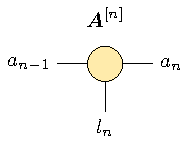
\includegraphics[]{figures/tikz/mps/basic/single_mps_tensor.pdf}}}.
\end{equation*}
\noindent Connecting lines of two tensors represents a contraction of these tensors along the specified legs.
A full MPS can be drawn by connecting the virtual legs of neighbouring tensors:
\begin{equation*}
    \vcenter{\hbox{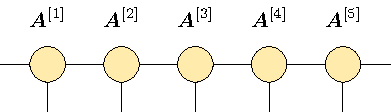
\includegraphics[]{figures/tikz/mps/basic/full_mps.pdf}}}.
\end{equation*}
\subsection*{Matrix Product Operators (MPO)}
After defining Matrix Product States it is a natural next step to also write operators in the MPS formalism. A general operator
$\hat{H}$ acting on the previously defined many-body system can be written as
\begin{equation*}
    \hat{H} = \sum_{l_1,l_2,\dots,l_N}\,\sum_{l_1^\prime,l_2^\prime,\dots,l_N^\prime}
    H_{l_1,l_2,\dots,l_N}^{l_1^\prime,l_2^\prime,\dots,l_N^\prime}
    \ket*{l_1, l_2, \dots, l_N} \bra*{l_1^\prime, l_2^\prime, \dots, l_N^\prime}
\end{equation*}
with the matrix elements $ H_{l_1,l_2,\dots,l_N}^{l_1^\prime,l_2^\prime,\dots,l_N^\prime}$. In the MPS formalism,
the operator becomes
\begin{equation}
    \label{eq:mpo}
    \begin{split}
        \hat{H} &= \sum_{l_1,l_2,\dots,l_N}\,\sum_{l_1^\prime,l_2^\prime,\dots,l_N^\prime} \sum_{j_0 = 1}^{\chi_0} \sum_{j_1 = 1}^{\chi_1} \cdots \sum_{j_{N-1} = 1}^{\chi_{N-1}} W_{j_0, j_1}^{[1], l_1, l_1^\prime} W_{j_1, j_2}^{[2], l_2, l_2^\prime}\cdots W_{j_{N-1}, j_0}^{[N], l_N, l_N^\prime} 
        \ket*{l_1, l_2, \dots, l_N} \bra*{l_1^\prime, l_2^\prime, \dots, l_N^\prime} \\
                &= \sum_{l_1,l_2,\dots,l_N}\,\sum_{l_1^\prime,l_2^\prime,\dots,l_N^\prime} \trace\left(
                    \vectorbold{W}^{[1],l_1,l_1^\prime} \vectorbold{W}^{[2],l_2,l_2^\prime} \cdots \vectorbold{W}^{[N],l_N,l_N^\prime}
                \right) \ket*{l_1, l_2, \dots, l_N} \bra*{l_1^\prime, l_2^\prime, \dots, l_N^\prime},
    \end{split}
\end{equation}
where the $\vectorbold{W}^{[n]}$ are tensors of rank four. Each of the tensors of the MPO has two physical and two virtual legs.
In the diagrammatic notation, an MPO can be written as
\begin{equation*}
    \vcenter{\hbox{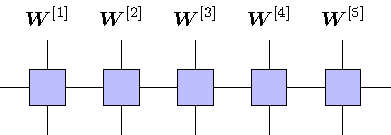
\includegraphics[]{figures/tikz/mps/basic/full_mpo.pdf}}}.
\end{equation*}